\section{LDPC over BSC}
\lecture{29. Apr}

Previously, we have studied how to decode an LDPC code over BEC. It is really a simple task, with the erasure density evolving acoording to \autoref{thm:w10_density_evolution}. However, if the decoding is over BSC, this task becomes much more difficult.

Consider the following figure, where we again consider the decoding of a $[3,6]$-LDPC.
\begin{figure}[H]
    \centering
    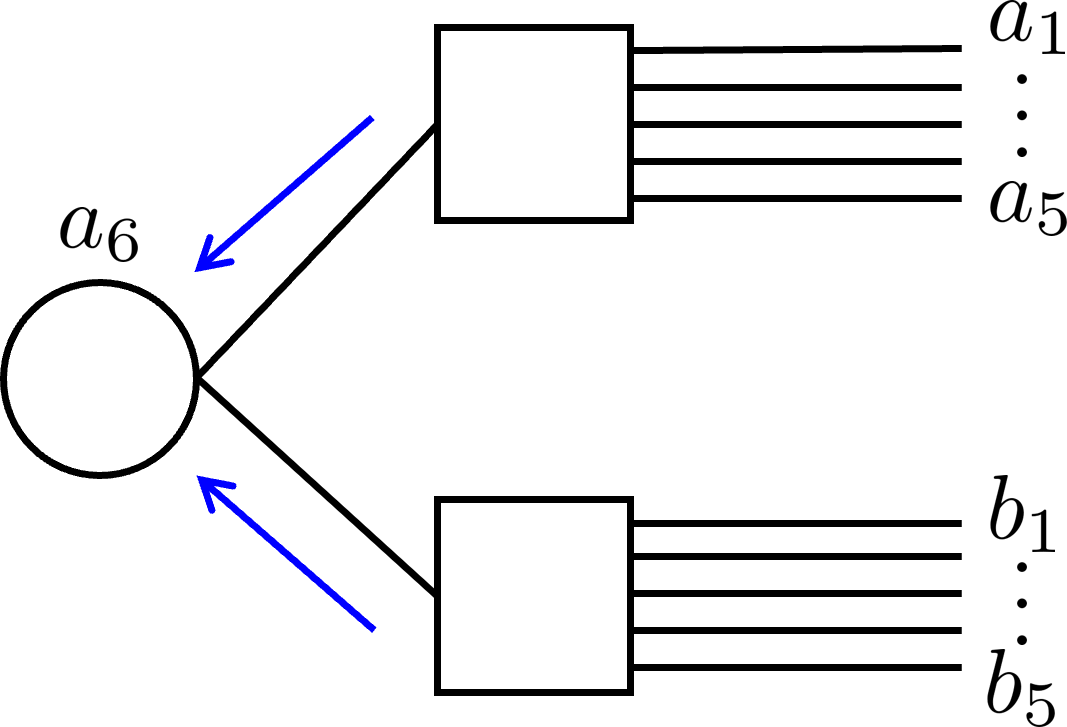
\includegraphics[width=0.3\linewidth]{figures/w11_LDPC_BSC.png}
    \caption{Belief propagation over BSC.}
    \label{fig:w11_belief_prop_BSC}
\end{figure}
If we propagate the value of $a_6$ directly from $a_1$ to $a_5$, then
\begin{equation*}
    a_6 = a_1 + \cdots a_5,
\end{equation*}
where the addition is over $\mathbb{F}_2$. However, there might be conflict with the lower branch of
\begin{equation*}
    a_6 = b_1 + \cdots + b_5.
\end{equation*}
One way to solve this conflict is by majority voting, where a variable node updates its value based on the suggestion that is the majority. However, this doesn't work in our case since both options are equally feasible.

A better method will be to utilize a \textit{soft decoder}.

\subsection{Gallager's Algorithm}
Instead of a strong decoder forcing a node to be an exact value causing major conflicts, we can use a soft decoder that \textit{suggests} the value a variable node should be.

For the following discussion, please also refer to \autoref{sec:w5_polar_dec_par_ser}, especially \autoref{thm:w5_TV_multiply} and \autoref{eq:w5_LLR_add}. Each variable node, for example $\mathrm{VN}_i$ now carries the log-likelihood ratio (LLR) of value
\begin{equation}
    \mathrm{LLR}_i = \ln\frac{\mathrm{Pr}\{\mathrm{VN}_i=0\}}{\mathrm{Pr}\{\mathrm{VN}_i=1\}}.
\end{equation}
The LLR can also be transformed into the signed total variational distance (TV) via
\begin{equation}
    \mathrm{TV}_i = \tanh\left(\frac{\mathrm{LLR}_i}{2}\right).
\end{equation}
When the information are sent from $a_1,a_2,\ldots,a_5$ to $a_6$, the combined information is
\begin{equation}
    \mathrm{TV}_{a_6,a_{1:5}} = \prod_{i=1}^5 \mathrm{TV}_{a_i} = \tanh\left(\frac{\mathrm{LLR}_{a_6,a_{1:5}}}{2}\right). 
\end{equation}
However, information from the branch of $b_1,b_2,\ldots,b_5$ should also be considered. Combining with the original LLR that $a_6$ has, its updated LLR will be
\begin{equation}
    \mathrm{LLR}_{a_6,\text{new}} = \mathrm{LLR}_{a_6,\text{old}} + \mathrm{LLR}_{a_6,a_{1:5}} + \mathrm{LLR}_{a_6,b_{1:5}}.
\end{equation}
The propagation and update of the probability of a VN being 0 or 1 is termed the belief propagation.

However, remember that the use of TV's and LLR's are just a matter of representation, and are only used since they are easy to combine under channel serial and parallel combination, respectively. For the example above, $a_6$ is originally a BSC. But after a single iteration of belief propagation, the $a_6$ channel updates to
\begin{equation}
    a_6 \ostar \left(a_1\boxstar\cdots\boxstar a_5\right) \ostar \left(b_1\boxstar\cdots\boxstar b_5\right).
\end{equation}

For a general LDPC over general channels, we have
\begin{theorem}[Density Evolution]
    Given an LDPC code with degree distributions from an edge perspective $\lambda(x)$ and $\rho(x)$. If the channel one communicates over with is $x_0=\mathcal{E}$, then through decoding, the equivalent channel updates according to
    \begin{equation}
        x_{n+1} = \mathcal{E}\ostar \lambda^{\ostar}\left(\rho^{\,\boxstar}(x_n)\right).
    \end{equation}
    The function $\lambda^{\ostar}$ is a polynomial with multiplication as parallel combination (equiv. to addition in the LLR representation); the function $\rho^{\,\boxstar}$ is a polynomial with multiplication as serial combination (equiv. to multiplication in the TV representation).
\end{theorem}

The step $\rho^{\,\boxstar}(x_n)$ worsens the channel, but the step $\mathcal{E}\ostar\lambda^{\ostar}(\ldots)$ improves the channel. As the iteration goes on, we would like to expect that $x_n\rightarrow \mathrm{BSC}(0)$ (the distribution over LLR goes to $\pm\infty$), then the LDPC code can be decoded as the quality of the bits becomes better and better, and the words converges to the correct codeword. If the distribution over LLR stays around zero, however, then we cannot decode the LDPC code. We can see whether decoding is possible or not given $\lambda$ and $\rho$ by plotting the EXIT chart.

\begin{figure}[H]
    \centering
    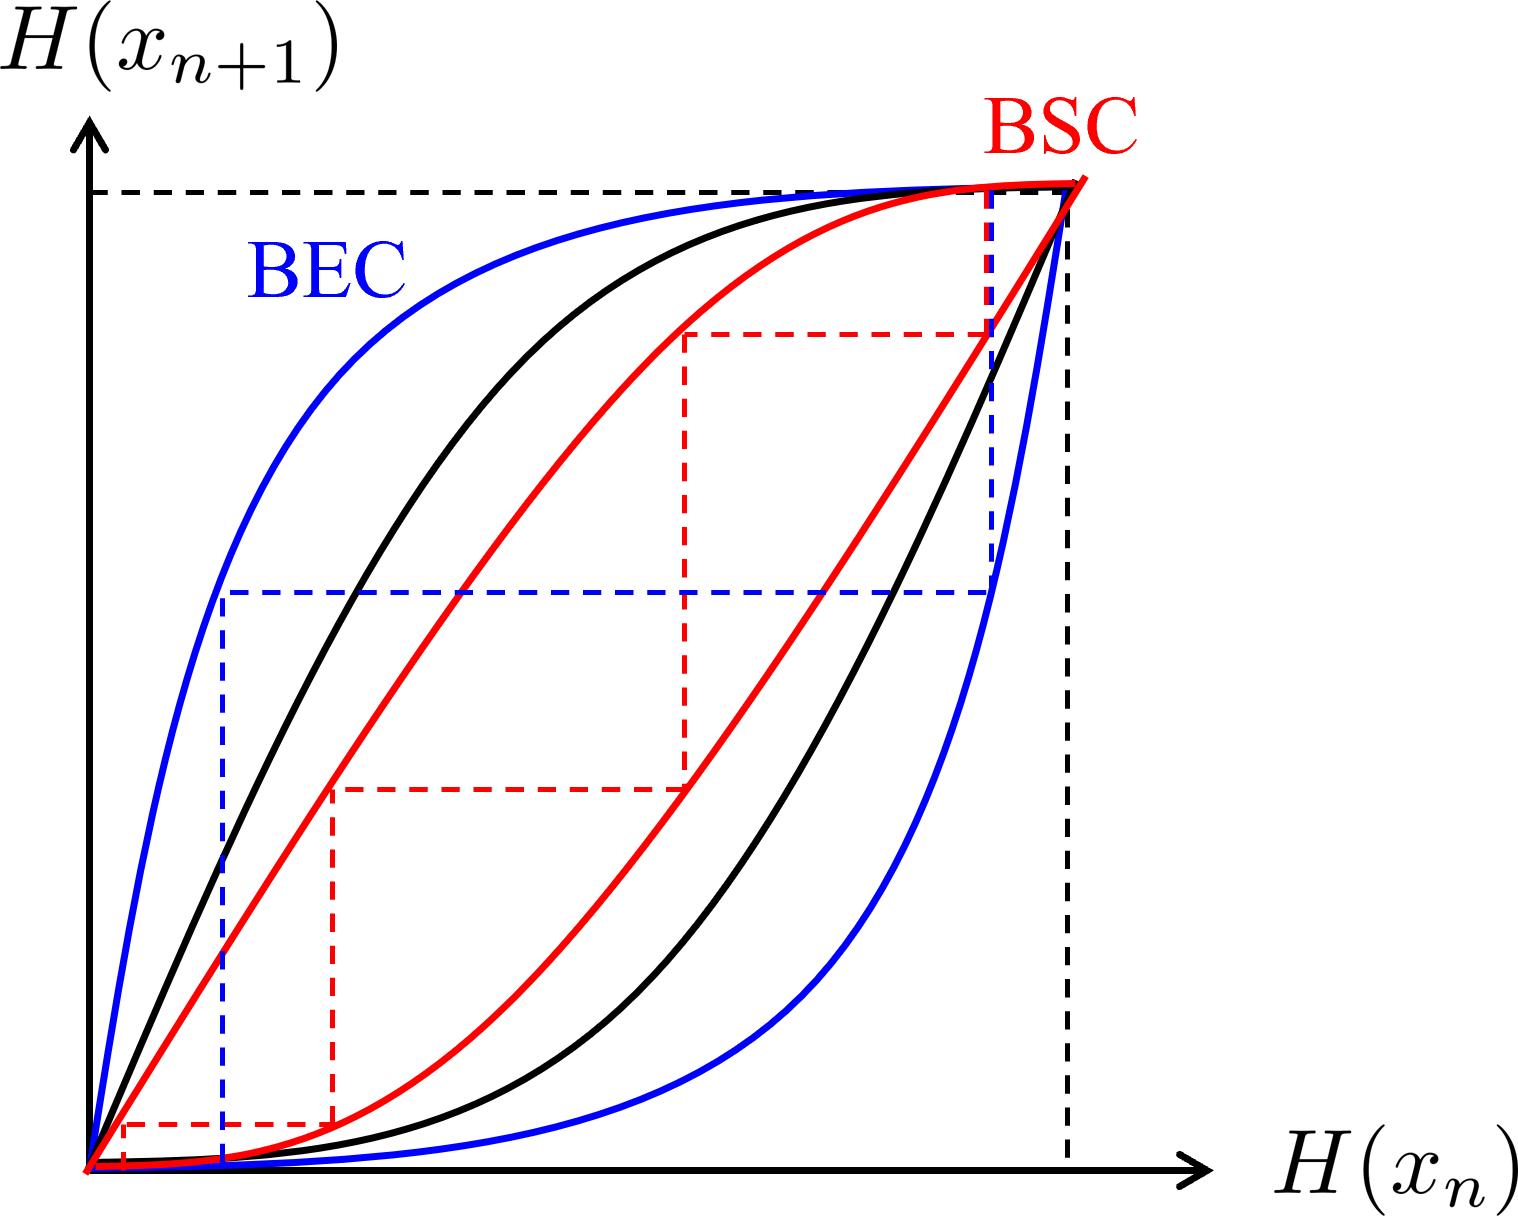
\includegraphics[width=0.5\linewidth]{figures/w11_EXIT.png}
    \caption{Illustration of the EXIT chart of LDPC code over general channels. The blue curves represent BEC, with the best performance; the red curves represent BSC, with the worst performance; the black curves represent any other channel, with intermediate performance.}
    \label{fig:w11_EXIT}
\end{figure}

See \autoref{fig:w11_EXIT}, we use the conditional entropy as an index of the channel quality. The two curves drawn is $(H(x_n),H(y_{n+1})$ and $(H(x_{n+1}),H(y_{n+1}))$, where
\begin{equation}\begin{aligned}
    y_{n+1} &= \rho^{\,\boxstar}(x_n),\\
    x_{n+1} &= \mathcal{E} \ostar \lambda^{\ostar}(y_{n+1}).
\end{aligned}\end{equation}

One can see that BEC converges faster to $(0,0)$ in comparison to BSC, and any other channel has performances in between the former two. Moreover, since the parallel and serial combination of both BEC and BSC remain as BEC and BSC, respectively, we can actually trace the dotted lines on the EXIT chart to see how the entropy evolves as one iterates the decoding scheme. This is not the case for other channels, however. For example, though the parallel combination of AWGN remains AWGN, the serial combination of AWGN becomes a different channel. Hence, one cannot use the EXIT chart to see how the channel conditional entropy iterates.

\begin{remark}
    Even though the serial combination of AWGN is not an AWGN, it is approximately one. Henceforth, as more of an engineering practice, we can assume it to be so and trace the evolution of the mean and variance of the channel output distribution. We can also argue the quality of the channel by seeing how the mean and variance evolve.
\end{remark}